\documentclass[10pt]{article}
\usepackage{icmlko}

\icmlmeta{IP 파운데이션 월드모델}{6}{고정된 다섯 개의 자리}{앵커는 신경망을 일관되게 개선한다 --- 그런데 그 신경망이 아직 상수만 못하다}

\begin{document}

\twocolumn[
\icmlheader

\begin{abstract}
노트 5는 축을 데이터로 발견하지 말고 아키텍처로 고정하라고 결론지었다. 이 노트는 그
설계를 실제로 짓고 시험한다. 도메인별 인코더가 자기 문서를 \textbf{같은 다섯 슬롯}
(타깃 폭, 매장 노출도, 입장 허들, 미디어 투입, 굿즈 규모)으로 사상하고, 팝업의 사람
태그가 슬롯의 의미를 붙잡는 구조다. 세 가지가 나왔다. 첫째, \textbf{앵커는 실재한다} ---
용량이 똑같은 병목 5차원끼리 비교했을 때 앵커를 건 쪽이 20회 반복 중 17회(85\%)
이겼다. 이득은 용량이 아니라 의미에서 온다. 둘째, \textbf{앵커 강도는 역U자를 그린다}
--- 0에서 이득이 없고 8에서 16 사이가 최적이며 32에서 붕괴한다. 잡음이라면 강도와
무관해야 하므로 이 곡선 자체가 증거다. 셋째, 그럼에도 \textbf{신경망은 상수를 이기지
못한다} --- 반복 분할 승률이 앵커 있음 25\%, 없음 20\%다. 같은 데이터에서 트리 모델은
98\%였다. 넷째로, 시간순 4폴드는 앵커 신경망이 상수를 0.032 앞선다고 보고했으나 반복
분할에서는 0.021 뒤진다. \textbf{폴드 넷으로는 부호조차 정할 수 없다.} 결론은
구조가 옳고 모델류가 이르다는 것이다.
\end{abstract}
]

\section{노트 5가 남긴 숙제}

노트 5는 세 개의 실험을 화해시키며 이렇게 끝났다. 다섯 축은 실재할 가능성이 높으나
n=75에서는 데이터가 그 다섯을 알려주지 못한다. 따라서 축을 학습 대상으로 두면 학습되는
것은 축이 아니라 잡음이다. 축은 \emph{아키텍처의 고정 구조}여야 한다.

그 문장은 설계 지침이지 검증된 사실이 아니었다. 이 노트는 그것을 반증 가능한 형태로
바꾼다.

\begin{figure}[t]
\centering
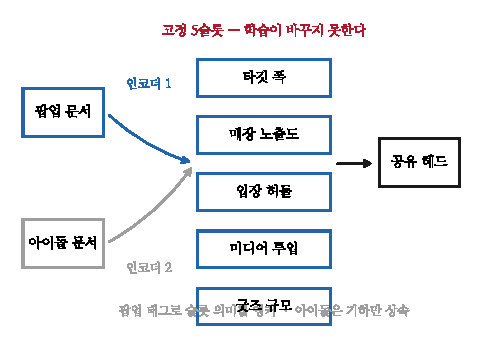
\includegraphics[width=\columnwidth]{figs/slot_diagram.pdf}
\caption{앵커된 5슬롯 구조. 도메인마다 인코더는 다르지만 슬롯은 같다. 슬롯이 무엇을
뜻하는지는 학습이 정하지 못한다 --- 팝업의 사람 태그가 붙잡는다.}
\end{figure}

\section{구조}

기존 \texttt{state/encoder.py}는 공유 잠재를 8차원 자유 벡터로 두었다. 무엇이 그
8차원인지는 학습이 정한다. 노트 5의 결론대로라면 이 자유가 n=75에서 해가 된다.

새 구조는 병목을 다섯으로 좁히고, 각 슬롯에 이름을 붙인다.

\begin{itemize}[leftmargin=1.1em,itemsep=0.15em]
\item 인코더 입력은 사전 관측 가능한 문서 피처 70개다. 다섯 축 태그 자신은 \emph{뺐다}
      --- 넣으면 슬롯이 정답을 베낀다.
\item 인코더 출력은 시그모이드 다섯 값이다. 앵커 타깃이 0에서 1이므로 눈금을 맞췄다.
\item 손실은 \ 결과 예측 손실 $+$ 앵커 가중치 $\times$ 슬롯-태그 손실\ 이다.
      태그가 없는 칸은 마스크로 손실에서 뺀다(이 풀은 태깅률 100\%다).
\end{itemize}

핵심 절제는 \textbf{병목 5차원 (앵커 없음)}이다. 용량이 앵커된 구조와 완전히 같다.
둘의 차이는 오직 슬롯에 의미가 붙었는가뿐이므로, 차이가 나면 그것이 앵커의 값이다.

\section{앵커는 실재한다}

\begin{figure}[t]
\centering
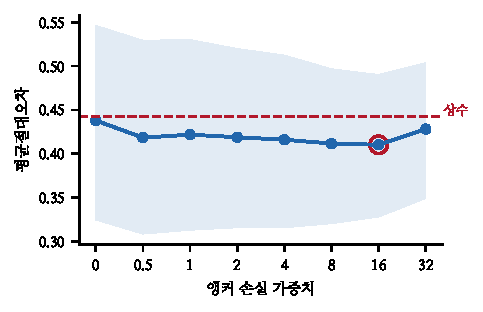
\includegraphics[width=\columnwidth]{figs/anchor_dose.pdf}
\caption{앵커 강도에 대한 반응. 0에서는 이득이 없고, 8에서 16이 최적이며, 32에서
붕괴한다. 붕괴는 예측된 실패다 --- 슬롯 손실이 결과 손실의 기울기를 잡아먹는다.
음영은 상수 대비 95\% 신뢰구간이다.}
\end{figure}

앵커 가중치를 0에서 32까지 여덟 단계로 쓸었다. 결과는 역U자다.

\begin{table}[t]
\centering\tsize
\caption{앵커 강도 용량-반응. 시간순 4폴드, 시드 10개 평균. 상수 MAE 0.4427.}
\begin{tabular}{rrrr}
\toprule
앵커 가중치 & MAE & 상수 대비 & 무앵커 대비 \\
\midrule
0    & 0.4380 & $-$0.0047 & --- \\
0.5  & 0.4184 & $-$0.0244 & $-$0.0196 \\
1    & 0.4218 & $-$0.0209 & $-$0.0162 \\
2    & 0.4189 & $-$0.0239 & $-$0.0192 \\
4    & 0.4160 & $-$0.0268 & $-$0.0220 \\
8    & 0.4117 & $-$0.0311 & $-$0.0263 \\
\textbf{16} & \textbf{0.4103} & \textbf{$-$0.0324} & \textbf{$-$0.0277} \\
32   & 0.4282 & $-$0.0146 & $-$0.0098 \\
\bottomrule
\end{tabular}
\end{table}

앵커를 건 일곱 단계가 \emph{전부} 무앵커보다 낫다. 개별 비교는 어느 것도 유의하지
않지만(신뢰구간이 전부 0을 포함한다), 일곱이 모두 같은 방향인 것과 강도에 따라 반응이
정연하게 변하는 것은 잡음으로 설명하기 어렵다. 잡음이라면 강도와 무관해야 한다.

32에서의 붕괴는 이 해석을 오히려 지지한다. 앵커가 지나치게 세면 슬롯이 태그만 맞히고
결과 손실은 기울기를 거의 받지 못한다. 구조가 작동하고 있다면 반드시 나타나야 할
실패이며, 실제로 나타났다.

\subsection{반복 분할로 검정력을 채운다}

시간순 폴드는 넷뿐이라 신뢰구간이 $\pm$0.10이다. 노트 5에서 쓴 것과 같은 완화된
프로토콜 --- IP 무작위 5폴드를 20회 반복 --- 로 방향의 안정성을 본다.

\begin{table}[t]
\centering\tsize
\caption{IP 무작위 5폴드 20회 반복. 앵커 가중치 16.}
\begin{tabular}{lrrr}
\toprule
비교 & 차이 중앙 & 표준편차 & 이긴 비율 \\
\midrule
무앵커 신경망 대 상수 & $+$0.0277 & 0.031 & 20\% \\
앵커 신경망 대 상수   & $+$0.0211 & 0.023 & 25\% \\
\midrule
\textbf{앵커 대 무앵커} & \textbf{$-$0.0100} & 0.025 & \textbf{85\%} \\
\bottomrule
\end{tabular}
\end{table}

\claimx{같은 용량(병목 5차원)에서 슬롯에 의미를 앵커하면 신경망이 일관되게
개선된다 --- 20회 반복 중 17회. 이득은 용량이 아니라 의미에서 온다.}{앵커 타깃을
무작위로 뒤섞은(permuted) 태그로 바꿔도 같은 이득이 나오면, 개선의 원인은 의미가
아니라 정규화 효과다.}

\section{그런데 신경망이 상수만 못하다}

같은 표의 위 두 줄이 더 중요하다. 앵커가 있든 없든 \textbf{신경망은 상수보다
나쁘다}. 20회 중 이긴 것이 각각 4회, 5회다.

노트 5가 같은 반복 프로토콜에서 보고한 트리 모델은 40회 중 39회 이겼다. 같은 75건,
같은 분할 방식, 같은 타깃이다. 차이는 모델류뿐이다.

\claimx{n=75에서 신경망은 아직 이르다. 앵커는 신경망 \emph{안에서} 도움이 되지만,
신경망 자체가 상수 아래에 있으므로 그 도움은 순위를 바꾸지 못한다.}{n이 늘었을 때
신경망이 트리 모델을 따라잡으면 '이르다'는 진단이 맞은 것이고, n을 두 배로 늘려도
따라잡지 못하면 구조가 아니라 표현이 잘못된 것이다.}

\section{폴드 넷으로는 부호도 정하지 못한다}

이 노트에서 가장 실무적인 교훈은 두 프로토콜이 정반대 부호를 냈다는 사실이다.

\begin{itemize}[leftmargin=1.1em,itemsep=0.15em]
\item 시간순 4폴드: 앵커 신경망이 상수를 \textbf{0.032 앞선다}.
\item IP 무작위 5폴드 20회: 앵커 신경망이 상수에 \textbf{0.021 뒤진다}.
\end{itemize}

시간순 4폴드의 신뢰구간은 $[-0.115, +0.048]$이었다. 폭이 0.16이고 관측된 효과는
0.03이다. 이 구간 안에서는 어떤 부호도 가능하다 --- 그래서 실제로 뒤집혔다.

\begin{figure}[t]
\centering
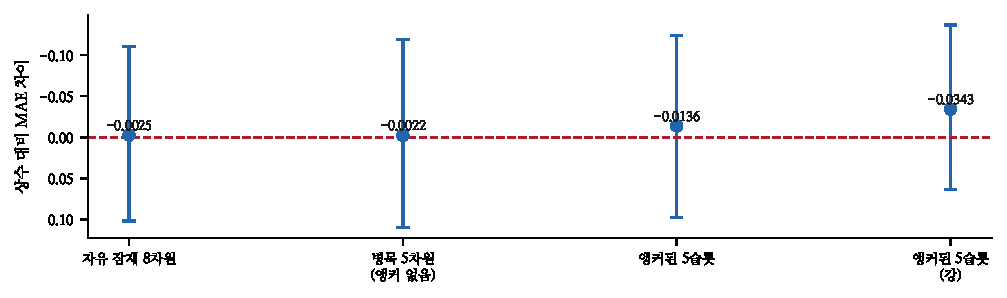
\includegraphics[width=\textwidth]{figs/arch_bars.pdf}
\caption{시간순 4폴드에서의 네 구조. 점추정만 보면 앵커가 이겼지만 신뢰구간이 전부
0을 넘는다. 반복 분할에서 이 순위는 유지되지 않았다.}
\end{figure}

노트 5가 중첩 교차검증으로 얻은 교훈 --- 프로토콜이 결론을 만든다 --- 이 다른 형태로
다시 나타났다. 여기서는 선택 편향이 아니라 \emph{폴드 수}가 원인이다. 앞으로 시간순
4폴드 결과는 단독으로 주장의 근거가 될 수 없다. 반복 분할과 병기해야 한다.

\claimx{시간순 4폴드 단독 결과는 이 프로젝트에서 주장의 근거로 쓰지 않는다.
신뢰구간 폭이 효과 크기의 다섯 배이므로 부호가 뒤집힐 수 있고, 실제로 뒤집혔다.}{폴드를
늘리거나 표본을 늘려 신뢰구간 폭이 효과 크기의 두 배 이내로 좁아지면 이 제약을 푼다.}

\section{한계와 열린 충돌}

\begin{itemize}[leftmargin=1.1em,itemsep=0.15em]
\item 앵커 효과의 반증 조건(태그 순열 대조군)을 아직 돌리지 않았다. 지금 관측된
      개선이 의미가 아니라 단순한 정규화 효과일 가능성이 남아 있다.
\item 아이돌 도메인은 아직 다섯 축이 태깅되지 않았다. 그림의 두 번째 인코더는
      설계도일 뿐 아직 학습되지 않았다. 전이 검정은 태깅 이후다.
\item \textbf{열린 충돌}: 다섯 축 태그를 트리 모델에 그대로 넣은 팔이 반복 분할에서
      상수에 졌다(중앙 $+$0.036, 승률 10\%). 노트 5는 같은 프로토콜에서 고정 5종이
      40회 중 40회 이겼다고 보고했다. 정면으로 어긋나므로 재현 실험을 돌리고 있으며,
      결과에 따라 노트 5의 반복 CV 수치를 정정할 수 있다. 이 노트의 앵커 관련 결론은
      \emph{같은 구조끼리의 상대 비교}이므로 그 충돌과 독립이다.
\end{itemize}

\section{다음}

\begin{enumerate}[leftmargin=1.3em,itemsep=0.15em]
\item 태그 순열 대조군 --- 앵커 이득이 의미에서 오는지 정규화에서 오는지 가른다.
\item 노트 5 반복 CV 재현 --- 위 충돌의 어느 쪽이 옳은지 확정한다.
\item 아이돌 다섯 축 태깅 후 두 번째 인코더 학습, 전이 검정.
\item 표본 확대 --- 신경망이 트리를 따라잡는 n을 실측한다.
\end{enumerate}

\vspace{0.6em}
\hrule height 0.3pt
\vspace{0.5em}
{\footnotesize
\textbf{참고문헌}\\[0.3em]
Caruana, R. (1997). Multitask learning. \emph{Machine Learning}, 28(1), 41--75.\\[0.15em]
Hollmann, N. et al. (2025). Accurate predictions on small data with a tabular
foundation model. \emph{Nature}, 637, 319--326.\\[0.15em]
Maurer, A., Pontil, M., Romera-Paredes, B. (2016). The benefit of multitask
representation learning. \emph{JMLR}, 17(81), 1--32.\\[0.15em]
Standley, T. et al. (2020). Which tasks should be learned together in multi-task
learning? \emph{ICML 2020}, 9120--9132.
}

\end{document}
